\subsection{Procedure}
We started by placing a rail with position markers through a 200 loop coil. We then measured the diameter of the coil to be (20.7\,$\pm$\,5)\,cm and centered it at position $x=\SI{60 \pm 0.2}{\centi\metre}$. Afterwards, we placed our Pasco PS-2162, connected to a Pasco Airlink, on a cart which we then placed on the rail (see figure \ref{fig: Cart and rail}). We then started taking measurements every \SI{5}{\centi\metre} from $x=\SI{30}{\centi\metre}$ to $x=\SI{90}{\centi\metre}$. We first measured the background magnetic field and then measured the field while passing a \SI{0.34 \pm 0.01}{\ampere} current through the coil (measured with an analog ammeter). All measurements were taken over periods of at least \SI{5}{\second} at \SI{200}{\hertz}.

\begin{figure}
    \centering
    \includegraphics[width=0.5\linewidth]{figures/cart_and_rail.jpg}
    \caption{Pasco PS-2162 and Airlink setup on a cart on the rail with a 200 turn coil centered at $x=\SI{60 \pm 0.2}{\centi\metre}$}
    \label{fig: Cart and rail}
\end{figure}

\begin{figure}
    \centering
    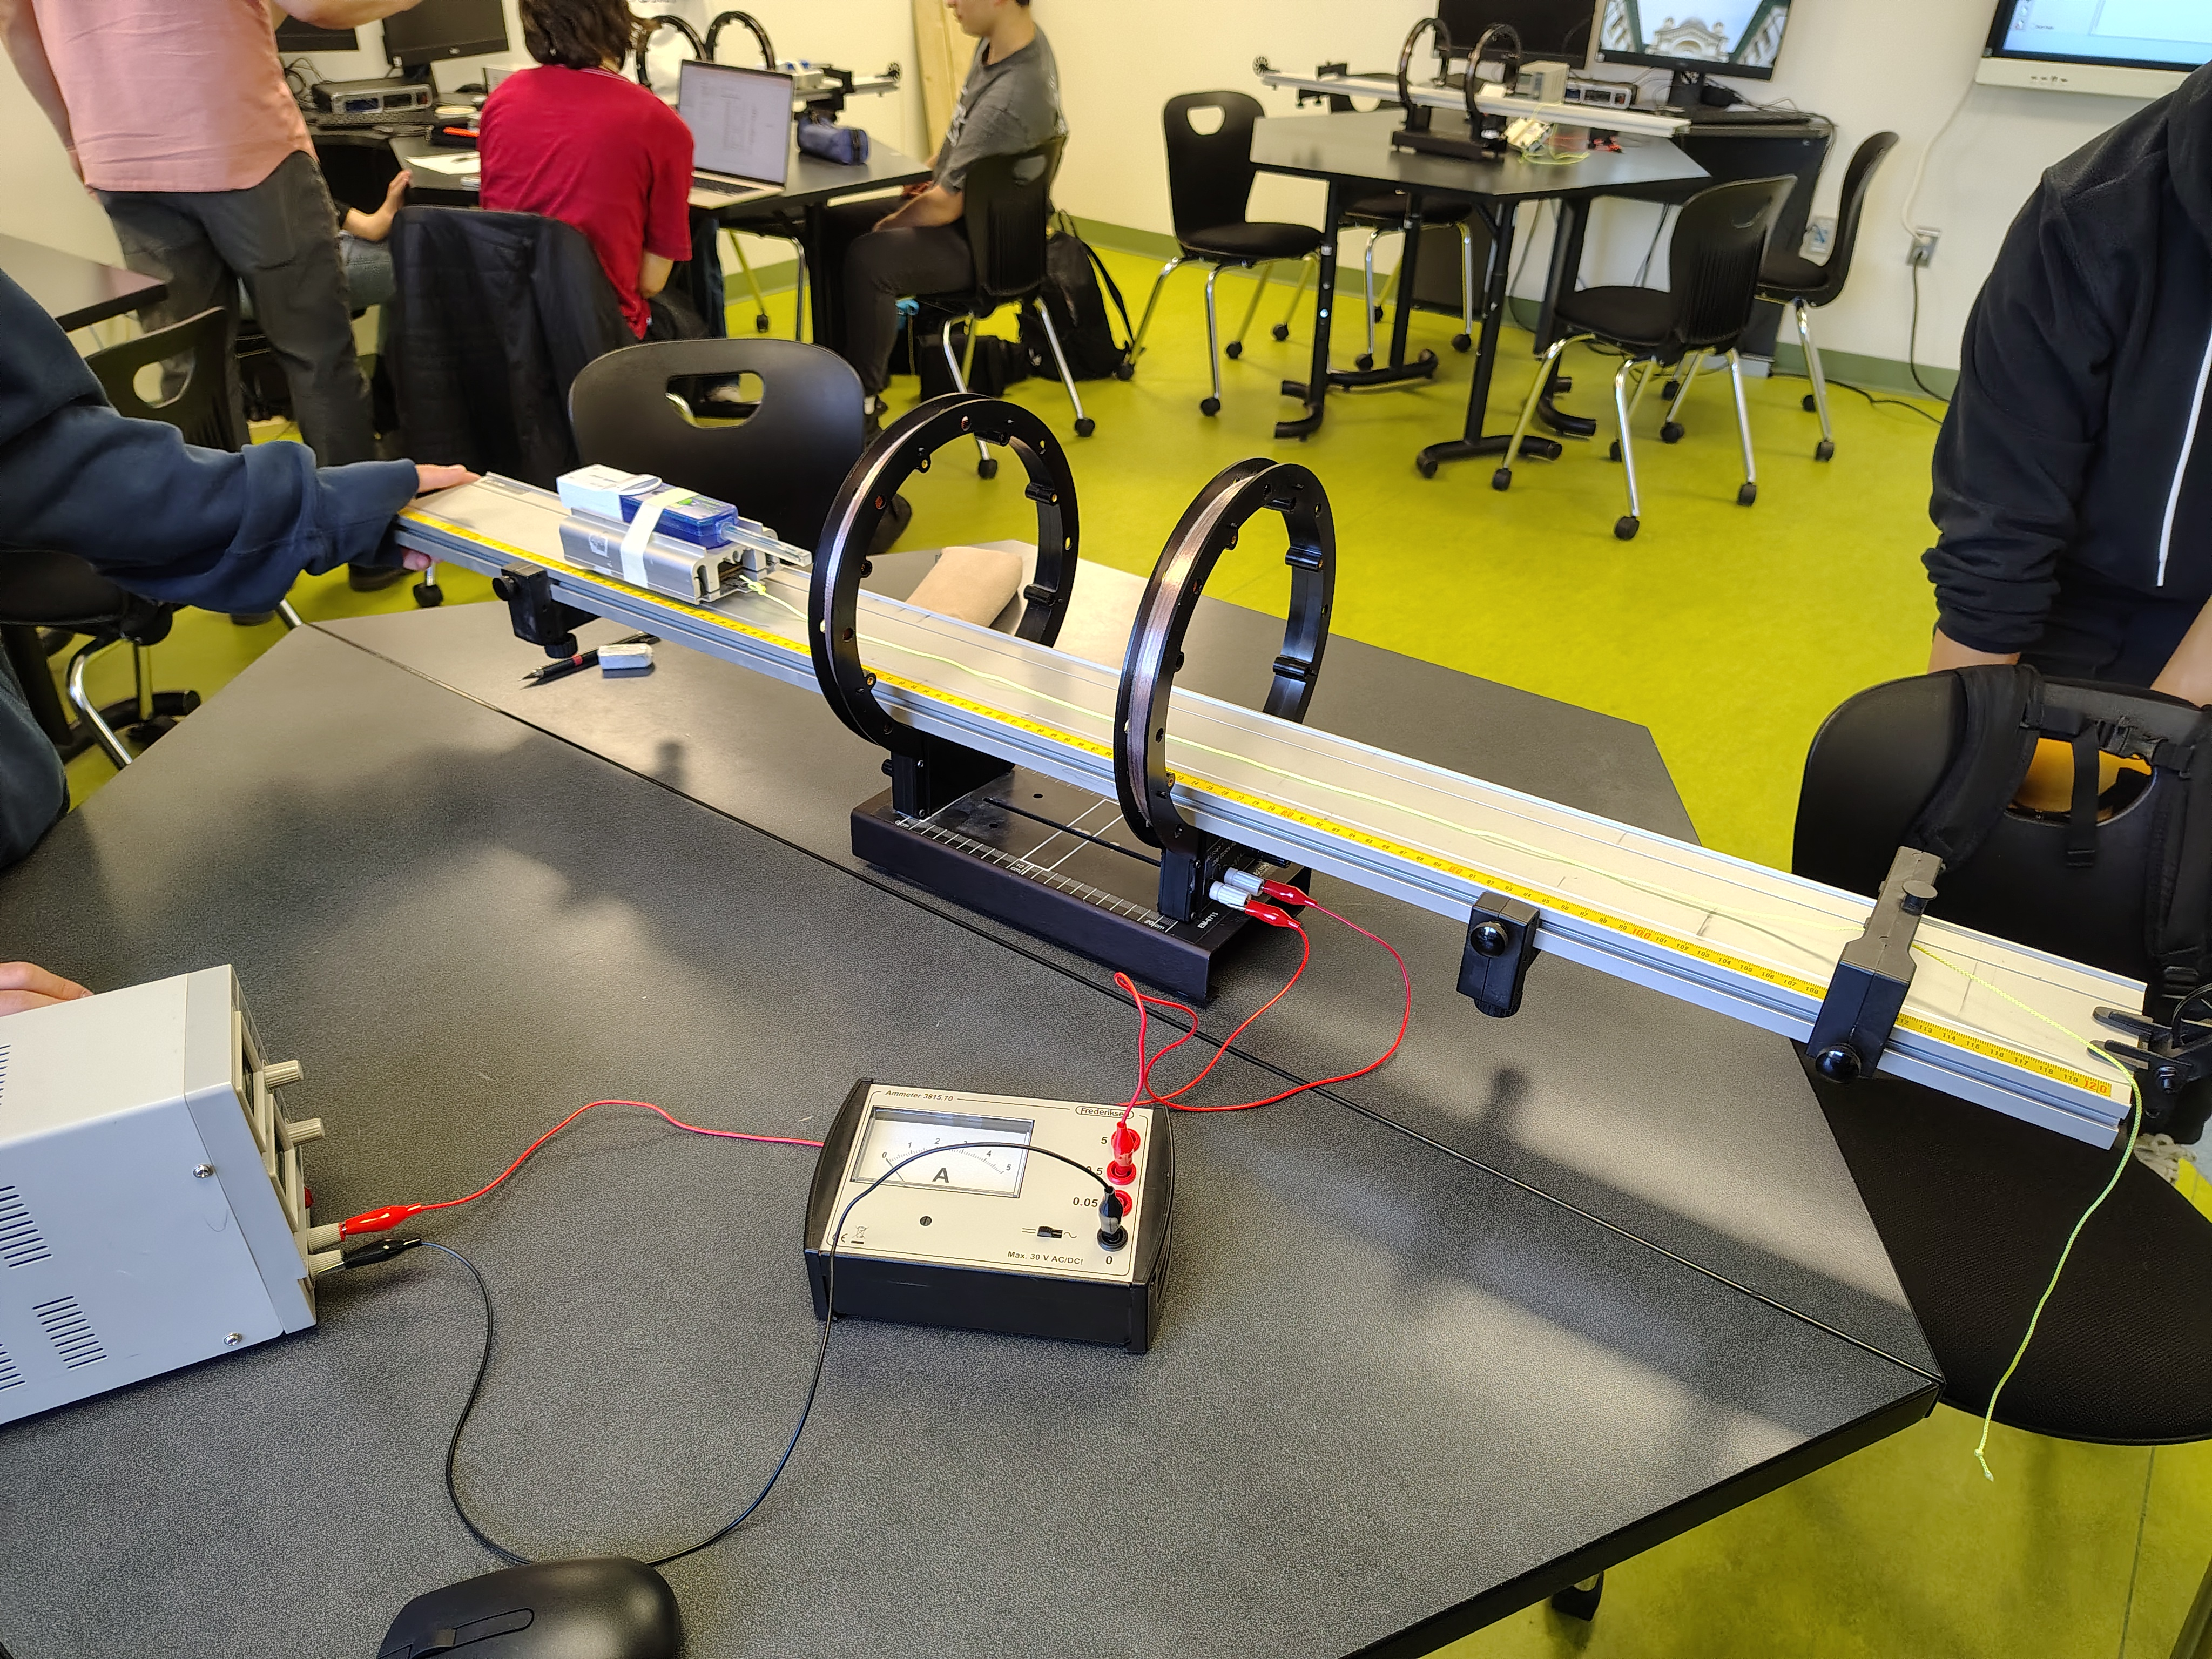
\includegraphics[width=0.5\linewidth]{figures/full_setup.jpg}
    \caption{Complete experimental setup. Power source on the left set to \SI{3.5}{\volt} and ammeter between the source and the rail.}
    \label{fig: Full setup}
\end{figure}

\subsection{Data}
We calculated the average measured magnetic field over intervals of 5 seconds. Any intervals that were longer than \SI{5}{s} were truncated to keep the data collection intervals consistent across all data points. Additionally, run \#10 of the background dataset was not used for the data analysis due to it being shorter than \SI{5}{\second}. The difference between the background and coil runs was calculated to find the magnetic field generated by the coil itself. We found that all measurements were within \SI{50.4}{\micro\tesla} of the expected values. All raw data can be found in the appendix and references\footnote{All data can be found \href{https://github.com/LudioRex/E-M_coil_lab}{here}.\\(https://github.com/LudioRex/E-M\_coil\_lab)}

\begin{table}[H]
\vspace{4mm}
\begin{tabular}{|c|c|c|}
\hline
\multirow{2}{*}{Postition (cm $\pm0.2$)} & Magnetic field     & Magnetic field     \\ 
       &            strength (G $\pm0.01$)   & strength (T $\pm 1$E-06)\\ \hline 
30     & 3.33E-01 & 3.33E-05 \\
35     & 2.55E-01 & 2.55E-05 \\
40     & 2.92E-01 & 2.92E-05 \\
45     & 6.29E-01 & 6.29E-05 \\
50     & 1.39E+00 & 1.39E-04 \\
55     & 3.20E+00 & 3.20E-04 \\
60     & 4.64E+00 & 4.64E-04 \\
65     & 3.48E+00 & 3.48E-04 \\
70     & 1.76E+00 & 1.76E-04 \\
75     & 7.20E-01 & 7.20E-05 \\
80     & 5.52E-01 & 5.52E-05 \\
85     & 4.72E-01 & 4.72E-05 \\
90     & 2.58E-01 & 2.58E-05 \\ \hline
\end{tabular}
\caption{Average magnetic field strength due to the current carrying coil at different positions along the coil's axis. Calculated by taking the difference between the measured background and the measured magnetic field with current flowing through the coil.}
\label{table: Averages}
\end{table}

\begin{table}[H]
\begin{tabular}{|c|c|c|}
\hline
\multirow{2}{*}{Postition (cm $\pm0.2$)} & Axial magnetic  & Relative \\
& field strength (T) & uncertainty (\%) \\ \hline
30 & 1.44E-05 & 44\% \\
35 & 2.32E-05 & 50\% \\
40 & 4.02E-05 & 57\% \\
45 & 7.58E-05 & 65\% \\
50 & 1.54E-04 & 70\% \\
55 & 3.02E-04 & 59\% \\
60 & 4.14E-04 & 15\% \\
65 & 3.02E-04 & 59\% \\
70 & 1.54E-04 & 70\% \\
75 & 7.58E-05 & 65\% \\
80 & 4.02E-05 & 57\% \\
85 & 2.32E-05 & 50\% \\
90 & 1.44E-05 & 44\% \\ \hline
\end{tabular}
\caption{Calculated expected values of magnetic field strength at different positions along the coil's axis.}
\label{table: Theoretical}
\end{table}

\pagebreak
\subsection{Calculations}
\begin{center}
    Note that the sample calculations may contain slight discrepancies with the data due to rounding errors.
\end{center}

\begin{center}
    \textbf{Sample Calculations for the distance from center}
\end{center}
\begin{align*}
    z&=\SI{0.60 \pm 0.02}{\metre}-\SI{0.30\pm0.02}{\metre}\\
    &=\SI{0.30 \pm 0.04}{\metre}
\end{align*}

\vspace{2mm}
\begin{center}
    \textbf{Sample calculations for the expected magnetic field strength}
\end{center}

\begin{align*}
    {B}_{\substack{\text{coil} \\ \text{on-axis}}} &= N\frac{\mu_0IR^2}{2(z^2+R^2)^{3/2}} \\
    &=\frac{200\cdot\SI{4\pi e-7}{\tesla\metre\per\ampere}}{2}\\
    &\times\frac{\SI{0.34 \pm 0.01}{\ampere}\cdot\left(\frac{\SI{0.207 \pm 0.05}{\metre}}{2}\right)}{\left((\SI{0.30 \pm 0.04}{\metre})^2+\left(\frac{\SI{0.207 \pm 0.05}{\metre}}{2}\right)\right)^{3/2}}\\
    &=\SI{1.26e-4}{\tesla\metre\per\ampere}\\
    &\times\frac{(\SI{0.34}{\ampere}\pm2.94\%)\cdot\left(\frac{\SI{0.207}{\metre}\pm2.42\%}{2}\right)^2}{\left((\SI{0.30}{\metre}\pm13.3\%)^2+\left(\frac{\SI{0.207}{\metre}\pm2.42\%}{2}\right)\right)^{3/2}}\\
    &=\SI{1.26e-4}{\tesla\metre\per\ampere}\\
    &\times\frac{(\SI{0.34}{\ampere}\pm2.94\%)\cdot(\SI{0.1035}{\metre}\pm2.42\%)^2}{\left((\SI{0.30}{\metre}\pm13.3\%)^2+(\SI{0.1035}{\metre}\pm2.42\%)^2\right)^{3/2}}\\
    &=\SI{1.26e-4}{\tesla\metre\per\ampere}\\
    &\times\frac{(\SI{0.34}{\ampere}\pm2.94\%)\cdot(\SI{0.0107}{\metre\squared}\pm4.84\%)}{((\SI{0.09}{\metre\squared}\pm26.6\%)+(\SI{0.0107}{\metre\squared}\pm4.84\%))^{3/2}}\\
    &=\SI{1.26e-4}{\tesla\metre\per\ampere}\\
    &\times\frac{\SI{3.64e-3}{\ampere\metre\squared}\pm7.78\%}{(\SI{0.09 \pm 0.02}{\metre\squared}+\SI{0.0170 \pm 0.0005}{\metre\squared})^{3/2}}\\
    &=\SI{1.26e-4}{\tesla\metre\per\ampere}\\
    &\times\frac{\SI{3.64e-3}{\ampere\metre\squared}\pm7.78\%}{(\SI{0.1071 \pm 0.0205}{\metre\squared})^{3/2}}\\
    &=\SI{1.26e-4}{\tesla\metre\per\ampere}\times\frac{\SI{3.64e-3}{\ampere\metre\squared}\pm7.78\%}{(\SI{0.1071}{\metre\squared}\pm19.2\%)^{3/2}}\\
    &=\SI{1.26e-4}{\tesla\metre\per\ampere}\times\frac{\SI{3.64e-3}{\ampere\metre\squared}\pm7.78\%}{\SI{0.035}{\cubic\metre}\pm28.8\%}\\
    &=\SI{1.26e-4}{\tesla\metre\per\ampere}\times(\SI{0.104}{\ampere\per\metre}\pm36.6\%)\\
    &=\SI{1.31e-5}{\tesla}\pm36.6\%\\
   % &=(1.3\times10^{-5}\pm5\times10^{-6})\,\text{T}
   &=\SI{13 \pm 5}{\micro\tesla}
\end{align*}

\begin{figure}[H]
    \centering
    \includegraphics[width = \linewidth]{figures/sets_graph_zoomed.png}
    \caption{Comparison of the two different measured data sets, background and coil+bkg, and the calculated coil magnetic field at different positions along the coil's axis.}
    \label{fig: Sets graph}
\end{figure}

\begin{figure}[H]
    \centering
    \includegraphics[width = \linewidth]{figures/measured_vs_theoretical_revised_zoomed.png}
    \caption{Measured magnetic field strength along the coil's axis compared to the expected values. Error bars represent uncertainty.}
    \label{fig: Measured vs theoretical}
\end{figure}

\begin{figure}[H]    \centering
    \includegraphics[width = \linewidth]{figures/perpendicular_sets_graph_revised.png}
    \caption{Comparison of the two different measured data sets, background and coil+bkg, and the calculated coil magnetic field perpendicular to the coil's axis at different positions along said axis.}
    \label{fig: Perpendicular sets graph}
\end{figure}

\vspace{1cm}
\subsection{Results}
Figure \ref{fig: Measured vs theoretical} shows the difference between the values we measured and those predicted by our model. Three of the points in this graph are outside the uncertainty range of the expected values, those being the points at $x\in\{\SI{30 \pm 0.2}{\centi\metre};\, \SI{85 \pm 0.2}{\centi\metre};\, \SI{90 \pm 0.2}{\centi\metre}\}$. These points were outside the range by \SI{12.5}{\micro\tesla}, \SI{12.4}{\micro\tesla}, and \SI{5.08}{\micro\tesla} respectively.